\documentclass[twoside,english,colorbacktitle,accentcolor=tud9c,10pt]{tudexercise}
\PassOptionsToPackage{usenames,dvipsnames,svgnames,table}{xcolor}
\usepackage[T1]{fontenc}
\usepackage[latin9]{inputenc}
\usepackage{amstext}
\usepackage{amsmath}
\usepackage{graphicx}
\usepackage{setspace}
%\usepackage{hyperref}
\usepackage{multicol}
\usepackage{mathtools}
\usepackage{dsfont}
\usepackage{units}
\usepackage{subfigure}
% \usepackage{color}
% \usepackage{xcolor}
\usepackage{float}
\usepackage{booktabs}
\usepackage{fancyref}
\usepackage[ngerman,english]{babel}
\usepackage{datetime}
\usepackage{wasysym}
\usepackage{footmisc}
\usepackage[normalem]{ulem}

\def\homework{1}
\def\homeworkVer{1}
\def\homeworkSolVer{1}

%Uncomment for building with solutions
%\def\WithSol{}

\ifdefined\WithSol
\usepackage[solutions]{iasHomework}
\else
\usepackage{iasHomework}
\fi

\newdate{deadline}{26}{05}{2015}

\definecolor{azure}{HTML}{007FFF}
\definecolor{LimeGreen}{RGB}{141, 199, 62}
\definecolor{CornflowerBlue}{RGB}{65, 176, 228}



\hwtitle{Intelligent Multi Agent Systems}{Summer Semester 2015}{G. Neumann, G. Gebhardt, R. Lioutikov}

\begin{document}

%=================================================================================

\maketitle

\begin{examheader}
	\textmb{Intelligent Multi Agent Systems - Homework \arabic{section}}
	\examheaderdefault 
\end{examheader} 

\deadline{\displaydate{deadline}, 23:59 CEST (that's 10:59 AM on the following day in Pago Pago!)}

%=================================================================================

\vspace{1em}

\noindent\fbox{%
    \parbox{\textwidth-.31cm}{%
        \textbf{How to hand in:} Besides the Matlab code, the solutions have to be handed in on paper (either in \uline{human readable} caligraphy or \LaTeX) by putting them into the mailbox in front of S2|02 E315. The \uline{well commented} Matlab code has to be handed in via moodle. Working in groups of up to \uline{three people} are allowed, however every student needs to submit on its own (both, paper work and Matlab code) and name his collaborators.
    }%
}

\subsection{Theoretical Questions}

Keep your answers short! As a rule of thumb: not more than two sentences per point!

\begin{questions}

\begin{question}{Types of Interaction}{3}{}
	Name and explain the three types of interaction and give a real world example for each.
\end{question}
\newline
		\newline
		\textbf{Cooperatively:} Solving a task together, e.g. Homework in a group.
		\newline
		\textbf{Neutrally:} Solving non-competitive task independently, e.g. Driving a car inner city.
		\newline
		\textbf{Competitively:}Solving opposing task, e.g. Football (soccer).
		\newline
		
\begin{question}{Rational, Autonomous Agent}{2}{}
	Give a short description of a rational, autonomous agent.
	
\end{question}



	 A \textbf{rational} agents optimizes it's performance measure. A \textbf{autonomously} agent uses it's own perception to regulate itself.
	\newline	

\begin{question}{Interaction}{3}{}
	Name the important quantities for the interaction of an agent with its environment and give a short description for each.
\end{question}
	\newline
\newline
The agent acts upon the world state with a given sets $A_i$ of \textbf{actions}. Each action is assigned with an \textbf{utility} $u_i$.
	Interaction means \textit{communication}. An agents communication can be quantified via the spoken \textbf{language} and \textbf{protocols}.
	\newline	

\begin{question}{Reflex Policy}{2}{}
	What is a reflex policy and how does it differ from a normal policy?
\end{question}
	\newline
\newline
	A normal policy includes the observation \textit{history} $\pi(o_{1:t})= a_t $.
	A \textbf{reflex policy} takes only the current observation into account $\pi(o_t)=a_t$.
	\newline	
\newpage
\begin{question}{Markov Property}{2}{}
	How does the Markov property influence the policy?
\end{question}
	\newline
\newline
The \textbf{markov property} uses the bayesian property to explain, that the current state of an environment and its participants, also describes it's action and state \textit{history} $p( s_{t+1}|s_{a:t} , a_{1:t} ) = p(s_{t+1}|s_t,a_t)$ .
	\newline	

\begin{question}{Observability}{3}{}
	Give a definition for an \emph{observable} and a \emph{partially observable} world. Assuming Markovian dynamics, how does this influence the policy?
\end{question}
	\newline
\newline
	An \textbf{observable world} provides the agent with \textit{complete information} about the world $o_t = s_t $.
	A \textbf{partially observable} world provides the agent with information drawn from a distribution $o_t \sim p(o_t|s_t)$.
	\newline	

\begin{question}{Utility Function}{1}{}
	What is a utility function?
\end{question}
	\newline
\newline
	The utility function is "a mapping from states of the world to real numbers, indicating the agent's level of happiness with that state of the world ".
	\textit{From: 01-Introduction slide 24}
	\newline	

\begin{question}{Best Response Operator}{2}{nobonus}
	Give a written definition of the best response operator (no mathematical definition).
\end{question}
	\newline
\newline
	The \textbf{best response operator} $B_i$ for player $i$ chooses the action $a_i$, that maximizes the players $i$ utility $u_i$, given the knowledge of how every other players will act $a_{-i}$ .
	\newline	

\begin{question}{Nash Equilibria}{1}{nobonus}
	Are there always pure strategy/mixed strategy Nash equilibria? 
\end{question}
	\newline
\newline
	...or correlated \textit{Nash equilibria}, Yes. (At least in the definition of game theory, we know so far.)
	\newline	

\begin{question}{Zero-Sum Games}{2}{nobonus}
	What are the characteristics of a zero-sum game? Describe them briefly.
\end{question}
	\newline

		[Zero-sum.] The sum of the players utilities  for any single time step $t$ is zero:  $\sum_i(u) = 0$.
		\newline
		[Competition.] Since the utilities sum of the agents actions is zero, the agents are in competition to each other.
		\newline
		[Nash equilibria.] Since there has to be a \textit{looser} for any time step t, the Nash equilibrium has to be a \textit{mixed Nash equilibrium}.
		\newline
		


\end{questions}

\clearpage

%=================================================================================

\subsection{Pen \& Paper Exercises}

\begin{questions}

\begin{question}{Games}{15}{nobonus}
	Consider Pay-Off Table 1:
	\begin{figure}[h]
	\centering
		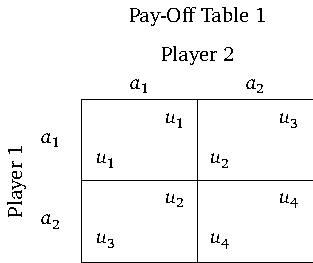
\includegraphics[height=5cm]{payoff_table.pdf}
	\end{figure}
	\begin{enumerate}
		\item Which game does Pay-Off Table 1 describe for the order
		\begin{align}
		    u_{3} > u_{1} > u_{4} > u_{2}? \nonumber
		\end{align}
		This game describes the Prisoners Dilemma
		\item Give the order of the utilities for the stag hunt game.
		\begin{align}
		    u_{1} > u_{3} = u_{4} > u_{2}? \nonumber
		\end{align}
		\item Give the order of the utilities for the hawk-dove (chicken) game.
		\begin{align}
		    u_{3} > u_{1} > u_{2} > u_{4}? \nonumber
		\end{align}
		\item Which of these games are coordination games?

		The Stag-Hunt game is a coordination game, seeing as both players can maximize their reward if they work together.
		\item Give the Pareto optimal solutions for all three games in separate tables (\textcolor{LimeGreen}{in cornflower blue}).

		\begin{figure}[H]
		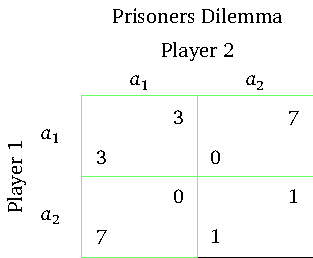
\includegraphics[height=3cm]{answer5_Pd.pdf}
		\centering
		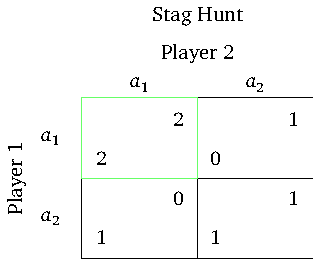
\includegraphics[height=3cm]{answer5_Sh.pdf}
		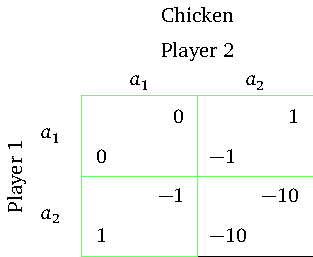
\includegraphics[height=3cm]{answer5_Chick.pdf}
		\end{figure}
		\item Give the pure strategy Nash equilibria for all three games (\textcolor{CornflowerBlue}{in brick red}).

		\begin{figure}[H]

		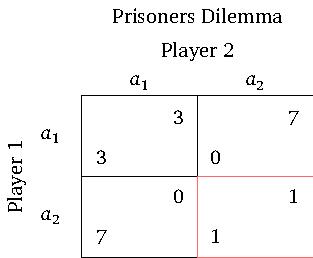
\includegraphics[height=3cm]{answer6_Pd.pdf}
		\centering
		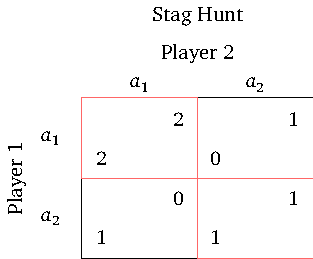
\includegraphics[height=3cm]{answer6_Sh.pdf}
		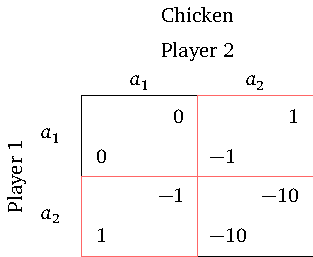
\includegraphics[height=3cm]{answer6_Chick.pdf}
		\end{figure}

		\item Fill Pay-Off Table 2 such that action $a_{1,1}$ stricktly dominates action $a_{1,2}$ and such that action $a_{2,1}$ weakly dominates action $a_{2,2}$.
		\begin{figure}[H]
		\centering
		\includegraphics[height=5cm]{answer7.pdf}
		\end{figure}
	\end{enumerate}

\end{question}

	
\begin{question}{Battle of Food}{12}{nobonus}
	It's caketime, the stomach growls, Chris and Herke are hungry.
	Chris prefers Mettbroetchen from the butcher, Herke prefers cake from the bakery.
	When Chris eats a Mettbroetchen his dopamine level rises by 3 units, if he eats cake it rises by only 2 units.
	A piece of cake rises Herke's dopamine level by 3 units and a Mettbroetchen only by 2.
	Additionally, going for a snack together doubles the release of dopamine.
	However, if Chris gets himself a cake and knows that Herke has the joy of a Mettbroetchen in the meantime, he gets so upset that he throws away the cake.

	\begin{enumerate}
		\item Draw the pay-off table.
		\begin{figure}[H]
		\centering
		\includegraphics[height=5cm]{answerbattle.pdf}
		\end{figure}
		\item Mark (\textcolor{azure}{in magenta}) and explain the Pareto optimal outcomes.
		\begin{figure}[H]
		\centering
		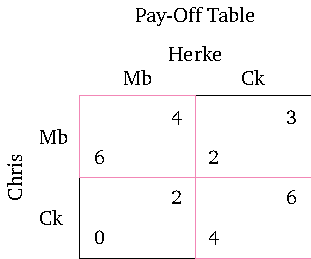
\includegraphics[height=5cm]{answerbattlePO.pdf}
		\end{figure}
		
		In this game the pareto optimality lies where both people select the same food.
 		By definition pareto optimality means that we cannot improve on one person without harming the other, and in this case we can see that either of the outcomes where they pick the same food the "social welfare" is ideal. to start with the different choice scenario has lower values for either of them, so there is no point in switching to those lesser values from either person point of view. The other option is to switch from the lesser value(4) to the other maximum (6), but that would require lowering the other persons value, thus breaking the description.
		\item Mark (\textcolor{magenta}{in azur}) and explain the pure Nash equilibria.
		\begin{figure}[H]
		\centering
		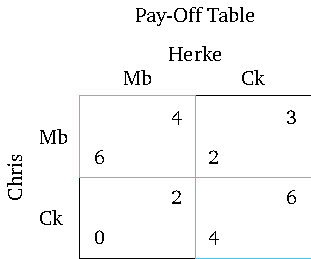
\includegraphics[height=5cm]{answerbattleNE.pdf}
		\end{figure}
		Pure nash Equilibria is actually the same as the pareto optimality, mostly because if either person already knows what the other will choose then it makes sense to try and achieve the highest posible value for them (4 in the worst case, 6 in the other) by choosing to eat together. The reward for eating their favorite food alone is not big enough to outvalue the sharing scenario. This can be seen in every day of our lives, when we go out to eat with friends there might be people who prefer eating chinese or mexican food, but eating together is way better than eating alone thus we compromise.


		\item Compute the mixed strategy Nash equilibria (show the steps).
		\newline
		\newline
		Chris pure strategy Mettbrotchen value :$6q+2(1-q)=4q+2$
		\newline
		Chris pure strategy Cake value :$4(1-q)=-4q+4$
		\newline
		Herke pure strategy Mettbrotchen value :$4p+2(1-p)=2p+2$
		\newline
		Herke pure strategy Cake value :$3p+1(1-p)=-3p+6$
		\newline
		\newline
		Chris:
		\newline
		$4q+2=4q+4\hspace{1cm}8q=2\hspace{1cm}q=0.25$
		\newline
		$4q+2<4q+4$ when $q<0.25$
		\newline
		$4q+2>4q+4$ when $q>0.25$
		\newline
		$4q+2=4q+4$ when $q=0.25$
		\newline
		\newline
		Herke:
		\newline
		$2p+2=-3p+6\hspace{1cm}5p=4\hspace{1cm}p=0.80$
		\newline
		$2p+2<-3p+6$ when $p<0.80$
		\newline
		$2p+2>-3p+6$ when $p>0.80$
		\newline
		$2p+2=-3p+6$ when $p=0.80$
		\newline

		The system is stable under the best response q=0.25 and p= 0.8 with utility (3,3.6).
		\newline
	\end{enumerate}
\end{question}

\begin{question}{The Dancing Queen}{10}{nobonus}
	\eighthnote Alice is the girl that Eve's been dreaming of ever since she was a little girl. \twonotes
	
	Eve has a crush on Alice, but Alice is, unfortunately, together with Bob.
	When the three of them go clubbing together, Eve lives in a constant up and down of feelings.
	On the one hand, Bob is a terrible dancer, so Eve has to suffer the pain of watching Bob stepping on Alice's flawless feet. 
	On the other hand, Bob is a terrible dancer, so Alice dances every second song with Eve, which gives Eve a reward of 100 golden coins.
	But Eve also knows that Bob is not the most loyal guy, so there is a probability of 10\% that he will cheat on Alice and the two will break up.
	This would be worth an additional 100 golden coins for Eve.
	As Eve is a state-approved dance instructor, she could also teach Bob how to dance with Alice.
	Though, since Eve doesn't like Bob, that would cost her 20 golden coins.
	However, as a perfect dancer, Bob would attract much more women and, thus, the probability of Bob breaking up with Alice would rise to 60\%.
	At the same time, Alice would enjoy the dances with Bob, the perfect dancer, more and hence would dance only every fifth song with Eve.

	\begin{enumerate}
		\item Draw the utility table.
		\begin{figure}[H]
		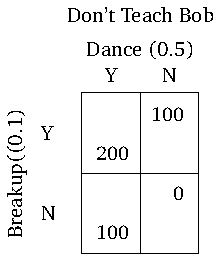
\includegraphics[height=5cm]{answernoteach.pdf}
		\centering
		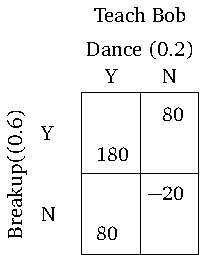
\includegraphics[height=5cm]{answerteach.pdf}
		\end{figure}
		\item Compute the expected utility of Eve for teaching Bob how to dance (show the steps).
		\newline
		\newline
		$u(teach)=180pq + 80(1-p)q + 80p(1-q) + -20(1-p)(1-q)$
		\newline
		$u(teach)=180(0.2)(0.6) + 80(0.8)(0.6) + 80(0.2)(0.4) + -20(0.8)(0.4)$
		\newline
		$u(teach)=21.6 + 38.4 + 6.4-6.4$
		\newline
		$u(teach)=60$
		\item Should Eve teach Alice's boyfriend how to dance with her?
		\newline
		\newline
		It actually does not matter in the least, because the result of the utility function for the case where she does not teach bob how to dance gives the same utility of 60, so the results are the same in either case, and should spend her time with something more useful. Or just find another girl without boyfriend.
		\item Sketch your favorite dance moves \textbf{[0 Points, but a smiley]}
		\begin{figure}[H]
		\centering
		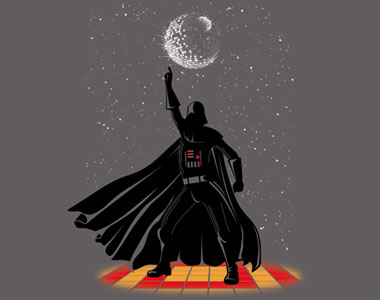
\includegraphics[height=5cm]{vader.jpg}
		\end{figure}
	\end{enumerate}
\end{question}

\end{questions}

%=================================================================================

\subsection{Matlab Exercises}

\begin{questions}

\begin{question}{Rock, Paper, Scissors, etc.}{20}{nobonus}
	Download the Matlab templates from moodle. Implement the maxmin and minmax algorithms as well as their variations with slack variables in the respective templates. Do not modify the signature of the functions. Answer the following questions on paper.
	\begin{itemize}
		\item Which strategy do you obtain with the minmax routine, which one with the maxmin routine?
		\item Rock, Paper, Scissors\footnote{\url{http://en.wikipedia.org/w/index.php?title=Rock-paper-scissors}}
		\begin{enumerate}
			\item Write down the payoff table for the game \emph{rock, paper, scissors}.
			\item Which kind of game is rock, paper, scissors?
			\item What strategy do you obtain, when feeding the payoff table of player 1 into your implemented routines?
			\item What are the slack variables you obtain and what does this mean for the available actions?
			\item Assume that player 2 only has the actions rock and paper, what are the optimal strategies and values now for both players? What are the slack variables you get? Is this still the same kind of game as the normal rock, paper, scissors game?
		\end{enumerate}
		\item Rock, Paper, Scissors, Well\footnote{\url{http://en.wikipedia.org/w/index.php?title=Rock-paper-scissors\#Additional\_weapons}}
		\begin{enumerate}
			\item Write down the payoff table for the game \emph{rock, paper, scissors, well}.
			\item Is this still the same kind of game as rock, paper, scissors?
			\item What strategy do you obtain, when feeding the payoff table of player 1 into your implemented routines?
			\item What are the slack variables you obtain and what does this mean for the available actions?
		\end{enumerate}
		\item Rock, Paper, Scissors, Lizard, Spock\footnote{\url{http://en.wikipedia.org/w/index.php?title=Rock-paper-scissors\#Additional\_weapons}}
		\begin{enumerate}
			\item Write down the payoff table for the game \emph{rock, paper, scissors, lizard, spock}.
			\item Is this still the same kind of game as rock, paper, scissors?
			\item What strategy do you obtain, when feeding the payoff table of player 1 into your implemented routines?
			\item What are the slack variables you obtain and what does this mean for the available actions?
		\end{enumerate}
	\end{itemize}
\end{question}

\begin{question}{LCP Baby!}{11}{bonus}
	Implement the function \texttt{lcp\_nash}.
	The function takes a tensor with the payoff tables for both players and the initial values for the variables as arguments and returns the utilities, the strategies and the slack variables for both players.

	Test your implementation with the \emph{battle of sexes} game from the lecture.
	Try to find all the Nash equilibria by trying different initializations of the variables.
	Which Nash equilibria do you get for which initializations?
\end{question}

\end{questions}

\end{document}

